%%=================================================
%% chapter01.tex for BIT Master Thesis
%% modified by yang yating
%% version: 0.1
%% last update: Dec 25th, 2016
%%==================================================
\chapter{绪论}
本章主要分为五部分,分别介绍了大数据高通量仿真和CPU/GPU并行计算的研究背景和意义,
CPU/GPU异构编程平台和GPU物理特性,最后介绍了本篇论文的主要研究工作和创新点。
\label{chap:intro}
\section{研究背景}
互联网技术的飞速发展颠覆了人们的传统生活方式,几乎每一个用户个体每天都会产生数
据,如何利用好这些海量数据成为各行各业急需解决的问题。大数据应用正融入生活的方
方面面,大数据计算用于建模与仿真学科也是必然的发展趋势。传统的单CPU处理器结构
计算能力有限,不适用于大数据仿真中,使用CPU/GPU异构计算才能快速处理大数据仿真。
大数据仿真中CPU/GPU异构计算的优化是本文研究的主要内容。

\subsection{大数据高通量仿真计算的研究背景和意义}
建模与仿真技术是以相似理论、模型理论、系统技术、信息技术,以及建模与仿真应用领
域的有关专业技术为基础,以计算机系统、与应用相关的物理效应设备及仿真器为工具,
根据对系统仿真的目标建立并利用模型对系统进行研究、分析、试验、运行和评估的一门
综合性、交叉性技术。建模与仿真技术和计算机科学一起,正成为继理论研究和实验研究之
后的第三种认识、改造客观世界的重要手段。大数据技术的出现给仿真技术带来了新的需
求与新的挑战,将大数据技术与仿真技术进行结合逐渐成为新的发展趋势。美国国防部高级
计划研究局于2012年发起1亿美元的XDATA计划,用于支持国防信息数据处理和
分析的软件和技术。军用仿真领域早在90年代就已经面临了大数据问题,美英1997
年联合举行的STOW97战争综合演练仿真,由500台计算机构成,超过3700个仿真实体参与,
在三个独立48小时阶段仿真中共计产生了大约1.5TB的数据。此后越来越多的军用仿真应
用不断出现,高解析模型甚至实装模型不断运用到仿真中,仿真产生的数据也在快速增长
。但是由于计算能力、计算方法等各种原因,仿真采集的绝大部分数据被丢弃了,仿真数
据的使用多处于仿真结果检查或者简单统计分析的级别,没有起到军事分析、决策和预测
的作用。国内外仿真专家近年不断探讨大数据与仿真的结合方式,试图寻求新的建模与仿
真方法。有学者提出大数据时代基于仿真的工程科学还需要发展仿真范式, 实现密集计算
与密集数据的集成,以实现无组织复杂系统因果规律的发现。数据密集方法可由数据从整
体上分阶段发现涌现性、演化机制下的结果, 而计算密集方法在部分时段或部分区域上满
足了相似性研究的需要,为实现整体上的可预测性,即通过模型运行来揭示相应复杂性系
统的运行规律,必须将数据密集与计算密集集成起来。这就是大数据高通量仿真要解决的
核心问题之一。数据量较少的仿真实验很多情况下是不足以描述事物发展趋势的,海量的
实验数据可以更好的覆盖到实体各方面运行和结果参数,计算出其中的因果关系。传统的
单CPU处理器计算能力有限,不具备快速计算大数据仿真的能力。高性能异构集群协同计算
方法是解决数据密集且计算密集型大数据高通量仿真的首选方法。随着GPU和Intel至强Phi
等协处理器的不断发展,异构系统成为高性能计算的重要方式。将GPU与大数据处理框架集
成来解决数据密集且计算密集型大数据计算是近年的研究热点。

\subsection{CPU/GPU异构计算研究背景和意义}
GPU最初是被设计用于显卡中图形计算的,帮助CPU快速处理复杂的图像计算。由于其卓越的
并行计算能力,现在GPU不再只作用于显卡中,越来越多地作为协处理器帮助CPU处理高
并行的大数据计算。在一些专业的领域中,比如机器学习和生物研究中,CPU/GPU异构计算
的应用十分广泛。从CPU和GPU性质上看,CPU适合处理计算量比较小的逻辑运算,而GPU由于
其内部有很多个小的计算单元非常适合处理高度并行的复杂计算。单CPU
处理器结构的计算能力不足以满足海量数据的计算需求,因此业界普遍把GPU作为协处理器帮
助CPU处理高并行的大数据计算。特别是在大数据高通量的仿真程序中,大量的实验参数和仿真
计算必须依赖CPU/GPU异构计算才能快速得出实验结果。虽然GPU编程语言,如
CUDA、OpenAcc和C语言语法规则差别不是很大,语法也比较简单,但是GPU编程对于普通程序
员来说仍是一个巨大的
挑战。设计者只有清楚地了解GPU内部结构和CPU/GPU通信特点才能编写出高效地GPU程序。
首先,设计者需要人为判断哪些计算是数据量大,并行程度高,需要放到GPU中计算的。其次
CPU和GPU的内存是隔离的,在相应的处理器上计算时必须先把需要的数据拷贝到相应的内存中
,这需要程序员手动的设计CPU和GPU之间的数据交换过程。每一次GPU kernel的调用都涉及到
数据在CPU和GPU内存的交换,所以在有多个kernel的GPU程序中,数据在CPU内存和GPU内存之间
的反复拷贝将成为限制程序运行速度的一大障碍。
与此同时,我们也发现编译制导方式的CPU/GPU异构编程虽然能够很大
程度的降低GPU编程难度,但是由于CPU与GPU体系结构之间的差异和大数据高通量计算的数
据密集特点,要实现CPU/GPU高性能协同计算,难度仍然不小。正如在OpenAcc官方网站中介
绍的,由于使用了不同的编译制导语句控制CPU与GPU之间的数据通信,导致同一个算法性能
相差30倍。这主要是因为GPU内存带宽能够达到100GB/s\~{}250GB/s,平均为CPU内存带宽的
8倍,但是访问GPU显存却需要400\~{}800个周期,是访问内存十几倍,PCI-E总线的实际带宽也
只能达到8GB/s左右,CPU/GPU之间的I/O瓶颈问题已经是公认的阻碍CPU/GPU协同计算性能的
关键问题,这一问题对大数据高通量仿真的影响将更加明显。因此本论文拟研究面向大数据
高通量仿真的CPU/GPU异构计算数据通信模型与优化方法,以提高集群的大数据高通量计算能力。

\section{CPU/GPU异构编程简介}
大数据时代需要更加快速、更高并行的计算方式,使得GPU编程越来越普遍。业界普遍使用的GPU
编程语言有CUDA、OpenCL和OpenAcc,本节将对GPU编程语言做出简单介绍。另外,GPU编程
语言仅仅提供了操作GPU的计算语法,如何根据GPU物理结构去设计GPU计算来充分优化GPU计算
将在后续章节介绍。

\subsection{CUDA平台简介}
CUDA(Compute Unified Device Architecture),是显卡厂商NVIDIA推出的运算平台,一种
通用并行计算架构,支持Linux和Windows平台。该架构仅适用于NVIDIA显卡,已应用于GeForce、
ION、Quadro以及Tesla GPU上,使GPU能够快速解决
复杂的计算问题。它包含了CUDA指令集架构以及GPU
内部的并行计算引擎,开发人员现在可以使用C语言来为CUDA架构编写程序,
所编写出的程序可以在支持CUDA的处理器上以超高性能运行。CUDA3.0已经开始支持C++和FORTRAN。
从CUDA体系结构的组成来说,包含了三个部分:开发库、运行期环境和驱动。
开发库是基于CUDA技术所提供的应用开发库。目前CUDA的1.1版提供了两个标准的数学运算库——CUFFT
(离散快速傅立叶变换)和CUBLAS(离散基本线性计算)的实现。这两个数学运算库所解决的是典型
的大规模的并行计算问题,也是在密集数据计算中非常常见的计算类型。开发人员在开发库的基础上
可以快速、方便的建立起自己的计算应用。此外,开发人员也可以在CUDA的技术基础上实现出更多的开发库。
运行期环境提供了应用开发接口和运行期组件,包括基本数据类型的定义和各类计算、类型转换、内存管理、
设备访问和执行调度等函数。基于CUDA开发的程序代码在实际执行中分为两种,一种是运行在CPU上的宿主代
码(Host Code),一种是运行在GPU上的设备代码(Device Code)。不同类型的代码由于其运行的物理位置
不同,能够访问到的资源不同,因此对应的运行期组件也分为公共组件、宿主组件和设备组件三个部分,基
本上囊括了所有在GPGPU开发中所需要的功能和能够使用到的资源接口,开发人员可以通过运行期环境的编
程接口实现各种类型的计算。由于目前存在着多种GPU版本的NVidia显卡,不同版本的GPU之间都有不同的差异,
因此驱动部分基本上可以理解为是CUDA-enable的GPU的设备抽象层,提供硬件设备的抽象访问接口。CUDA提供
运行期环境也是通过这一层来实现各种功能的。目前基于CUDA开发的应用必须有NVIDIA CUDA-enable的硬件支持,
NVIDIA公司GPU运算事业部表示:一个充满生命力的技术平台应该是开放的,
CUDA未来也会向这个方向发展。由于CUDA的体系结构中有硬件抽象层的存在,因此今后也有可能发展成为一个通
用的GPGPU标准接口,兼容不同厂商的GPU产品。CUDA相比于其他GPU编程语言更加底层,需要程序员手动设计每次
GPU kernel 调用时的数据交换过程,这样可以使设计者根据需求充分利用GPU性能,同时也是对程序员的
一大挑战,不合理的GPU编程设计将会带来巨大的性能丢失。

\subsection{OpenCL简介}
OpenCL是第一个面向异构系统通用目的并行编程的开放式、免费标准,也是一个统一的编程环境,便于软件开发人
员为高性能计算服务器、桌面计算系统、手持设备编写高效轻便的代码,而且广泛适用于多核心CPU、GPU、Cell类型
架构以及数字信号处理器等其他并行处理器,在游戏、娱乐、科研、医疗等各种领域被广泛使用。OpenCL由一门
编写kernels的语言和一组用于定义并控制平台的API组成,提供了基于任务分割和数据分割的并行计算机制,支持
Windows和Linux操作系统。OpenCL 1.1标准支持三维矢量和图像格式等新数据类型,支持处理多Host指令以及跨设备的
缓冲区,并且通过链接OpenCL和OpenGL的事件,高效共享图像和缓冲区,大大改进了与OpenGL的互操作性。OpenCL对
图像格式的处理更加快速高效,也是图形学中常用的CPU/GPU异构编程语言之一。OpenCL 2.0在已有标准上首次引入
共享虚拟内存的支持,CPU和GPU内核可以直接共享复杂的,包含指针的数据结构,避免了程序员不熟悉异构编程造成的
冗余数据交换,大大提高了并行编程的灵活性。支持动态并行,GPU内核不需要与主句CPU交互情况下进行内核排队,
实现灵活的调度方式,减少数据在CPU内存和GPU内存之间的拷贝,降低CPU处理器的负担。该标准改进图像支持,内核
可以同时读写同一对象。新增对安卓系统的支持,安卓客户端可以安装驱动扩展将OpenCL作为共享对象进行操作。
OpenCL框架由平台API,运行时API和OpenCL编程语言组成。平台API用于宿主机程序发现OpenCL设备的相关函数和为OpenCL
应用创建上下文的相关函数。运行时API是用来管理上下文创建命令队列以及运行时的一些其他操作。OpenCL语言是用来
编写GPU内核计算代码的编程语言,与c语言相似。
目前主流的芯片厂商都已推出支持OpenCL的芯片,各大品牌的手机平板几乎全都能支持OpenCL。
移动端的GPU通用计算必然成为被广泛使用的技术,推动移动计算进入一个全新时代。


\subsection{OpenAcc简介}
OpenAcc是另一种面向CPU/GPU异构结构并行编程GPU编程语言。2011年11月,Cray、PGI、CAPS和英伟达4家公司联合
推出OpenACC 1.0编程标准,适用于NVIDIA和AMD显卡,支持Windowshe和Linux系统。
OpenAcc与CUDA和OpenCL相比,不需要程序员手动设计每一块数据在CPU和GPU内存之间的拷贝细节,
而是以一个或者多个在
GPU上执行的kernel为单位,以编译制导语句的方式告诉编译器在当前kernel的数据拷贝方式。OpenAcc大大降低了
GPU编程的门槛,很多数据的拷贝都是由编译器帮助程序员去完成的。程序设计者一般只需规划好哪些代码是在GPU上执行
和相应的编译制导语句就可以写出效率较高的OpenAcc程序。PGI编译器对OpenAcc的支持非常完善,GCC编译器也
支持大部分OpenAcc特性。使用CUDA重构C语言代码时,需要重写程序,OpenAcc并行化的方式不是重写程序,而
是在串行C/C++或Fortran代码上添加一些编译制导标记。支持OpenACC的编译器能够看懂这些标记,并根据标记含
义将代码编译成并行程序。对英伟达GPU来说,编译器将C/C++/Fortran代码翻译成CUDA C/C++代码,然后编译链接成并行程序。
对AMD GPU来说,中间代码是OpenCL。可见OpenAcc语言相比CUDA和OpenCL更加高级一点,不需要程序设计者
具体编写底层的数据拷贝语句,只需要程序员利用编译制导语句告诉编译器每个kernel的执行方式和数据拷贝。
程序耗时最多的是循环模块,OpenAcc把每个并行计算量很大的循环结构,看成是一个可以在GPU上执行的kernel。
循环结构中的迭代计算被分散到GPU上不同线程执行,GPU拥有多个核心可以同时快速运行多个线程,大大降低了CPU负担。
经上述章节介绍可以看出,无论选取何种GPU编程语言进行代码编写,都需要设计者规划那些计算需要在GPU上执行和每次
GPU kernel调用CPU内存和GPU内存之间的数据交换。本文的主要研究方向也是如何优化CPU内存GPU内存之间的数据交换来
优化GPU程序。

\section{GPU结构简介}
GPU作为协处理器,帮助CPU处理图形计算和一些其他的高并行的复杂计算,降低CPU负担,提高整个系统运行速度。
NVIDIA和AMD是现在最大的两个显卡供应商,本节就NVIDIA显卡的物理结构做出简单介绍,并且分析一些在CPU/GPU
异构计算中的一些瓶颈。
\subsection{CPU和GPU设计区别}
CPU和GPU的设计初衷打不相同,分别针对了两种不同的应用场景。CPU作为中央处理器需要很强的通用性来
处理各种不同数据类型,同时又要有处理判断循环等逻辑的控制结构,这使得CPU的内部结构异常复杂。而GPU的
设计初衷就是解决高度统一的、相互无依赖的大规模数据和不需要被打断的计算环境。图1是来自NVIDIA文档关于
CPU和GPU结构的描述图,其中绿色是计算单元,橙色是控制单元,蓝色是存储单元。从图中可以看出GPU内部有
大量的计算单元和超长的流水线,只有非常简单的控制逻辑并且cache,可见GPU的设计初衷就是用来处理大规模
数据计算的。相比GPU,CPU内部计算单元相对较少,被缓存占据了大量空间,拥有复杂的控制逻辑单元和诸多优化电路。
所以CPU的结构非常适合作为中央处理器来处理很多复杂的控制逻辑,同时大块的缓存也加速了对硬盘的读写,
但是由于计算单元有限不擅长计算大规模的并行计算。同时,GPU拥有很多的核心,可以快速并行运行多个线程,
处理循环时,在不破坏数据依赖的情况下可以把每一轮的迭代计算分散到不同线程上。
GPU拥有很少的cache,GPU缓存的目的是和CPU一样缓存后续可能使用到的数据,而是缓存线程需要的数据。
当有多个线程需要一个数据块时,GPU cache会合并这些请求,从DRAM中缓存这些数据到cache,然后再把GPU缓存中的
数据发送到相应线程。从上述描述可以看出,CPU作为中央处理器处理通用计算,负责和操作系统、硬盘、网络硬件等交互,
拥有复杂的逻辑控制单元可以快速处理每条指令。而GPU作为协处理器处理,是用来帮助CPU处理专用大规模数据的并行计算,
不需要与操作系统和其他硬件交互。
\begin{figure}
\centering
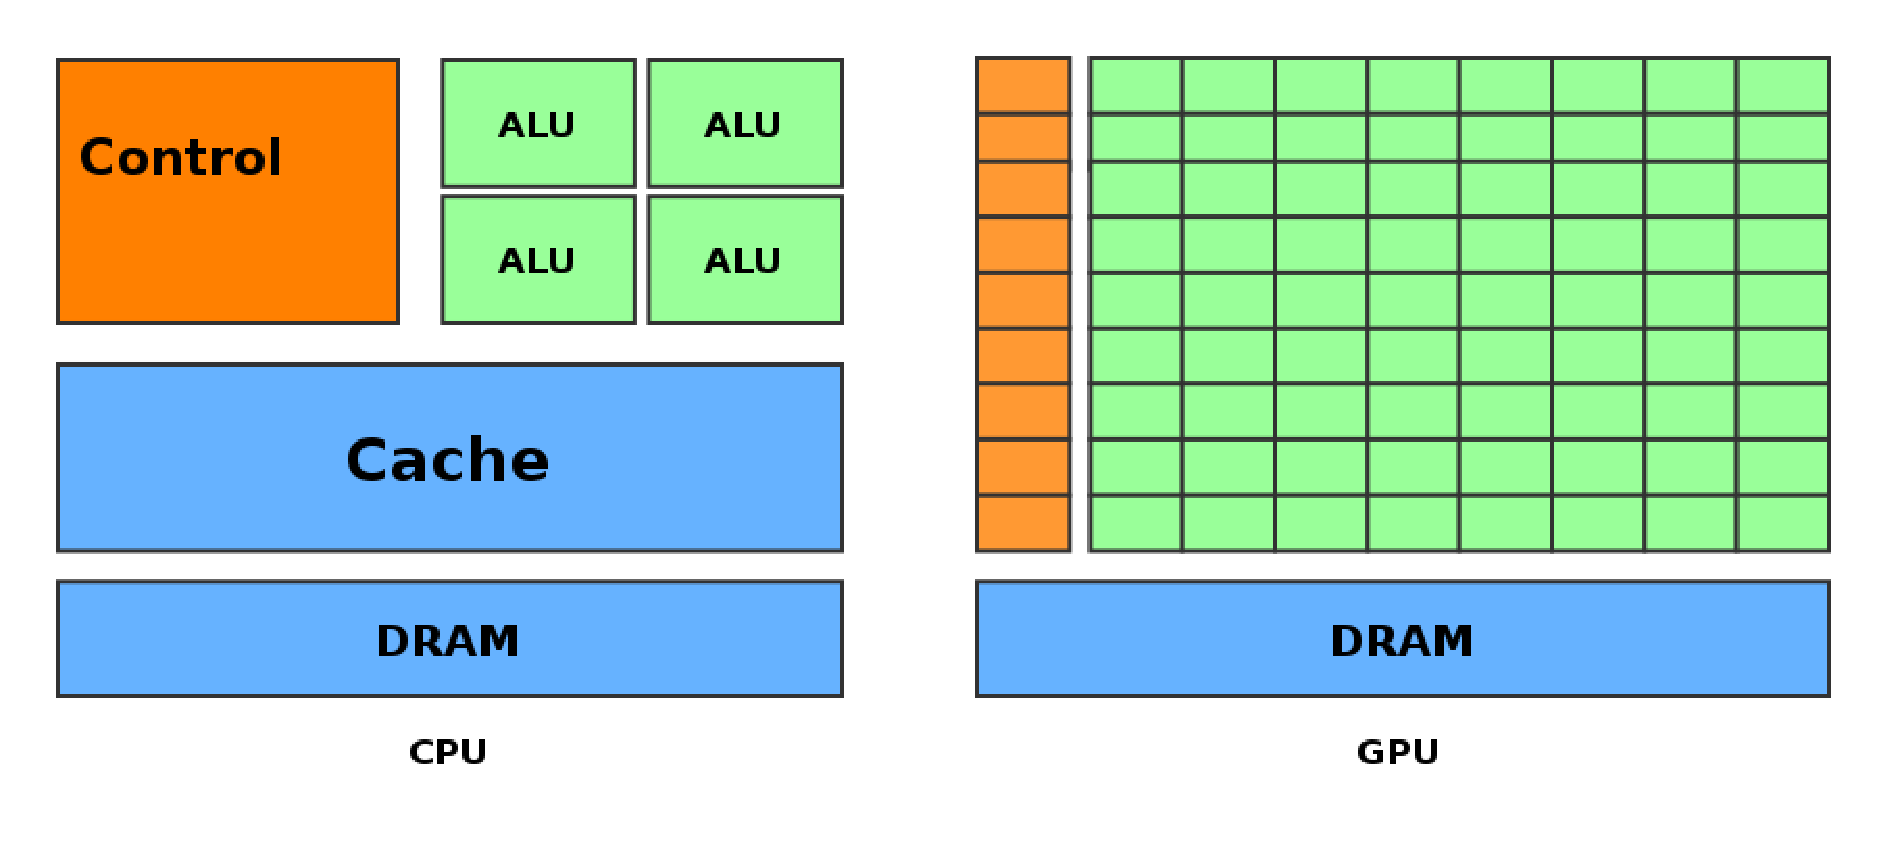
\includegraphics[width=0.9\linewidth]{figure1.eps}
\caption{CPU和GPU结构比较}\label{figure1}
\end{figure}




